\documentclass[8 pt]{article}
\usepackage[english]{babel}
\usepackage[utf8]{inputenc}
\usepackage{fancyhdr}
\usepackage{wrapfig}
\usepackage[margin=.7in]{geometry}
\usepackage{amssymb,amsmath,amsthm,mathrsfs}
\usepackage{graphicx}
\usepackage{caption}
\usepackage{mdframed}
 
\pagestyle{fancy}
\fancyhf{}
    \rhead{Origins Project Research Proposal}
\lhead{Shane M. Lubold}
\linespread{1}

\begin{document}


As our computing power inceases, questions that once seemed impossible to analyze become accessible. Faster computation has created new discoveries in economics, computer science, and engineering, but nowhere are these discoveries more important than in medicine. Biological processes, such as the growth of cancer, the spread of disease, or the evolution of species, are at the forefront of modern science. Answering these questions is crucial to our progress as a species. Reducing the time needed to model the growth of cancer, for instance, would translate into quicker diagnoses and faster, more effective treatments. Working under Dr. S\'{e}bastien Motsch in the School of Mathematical and Statistical Sciences, I plan to focus on three aspects of computational biology.

 Dr.\ Motsch and I are currently deriving an alternative to the traditional approach to modeling the behavior of biological systems. The traditional approach is to use differential equations to model such systems. For instance, 
a biologist interested in modeling cancer growth would try to solve:

\begin{equation}
\frac{\partial f}{\partial t} = D\Big(\frac{\partial^2 f}{\partial x^2} + \frac{\partial^2 f}{\partial y^2}\Big)+ f(1-f).
\label{eq: Macro}
\end{equation}

To solve such an equation, one discretizes the physical space (corresponding to the $x$ and $y$ variables) and the temporal space (corresponding to the $t$ variable). This approach requires the ratio $\frac{\Delta t}{\Delta x^2}$ to be very small in order for the solution to be accurate. This results in a computationally expensive problem. Furthermore, as the physical space gets larger, the computational time required increases exponentially. For problems of even moderate size, this approach is therefore impracticle.\\


\begin{wrapfigure}{L}{0.4\textwidth}
  \begin{center}
   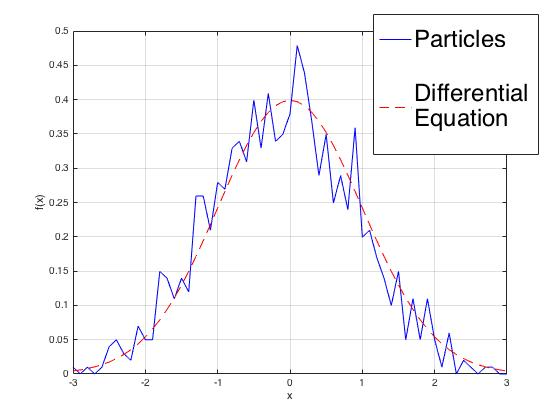
\includegraphics[width=0.4\textwidth]{OriginsPic.jpg}
  \end{center}
  \caption{Comparison of Approaches}
\end{wrapfigure} 

\noindent The second approach is to model the behavior of the physical system using particles. Instead of solving a complicated differential equation, one begins with a collection of particles, with $X_i^{m}$ denoting the $i$-th particle at time $m.$ One then computes the position of these particles at a future time with  
\begin{equation}
x_i^{m+1} = x_i^{m} + C\textbf{W},
\label{eq: Micro}
\end{equation}
where $C$ is a constant and $\textbf{W} \sim \mathcal{N}(0, 1).$ One simply needs to draw normally distributed numbers in order to approximate the behavior of the system. One can prove mathematically that these particles converge in distribution to the equation of the differential equation. In Figure 1,
the solutions from (\ref{eq: Macro}) and (\ref{eq: Micro}) are plotted.
This approach is computationally faster and places no restriction on the physical and temportal discretization, yet there is a problem. There has been little research done that computes the accuracy of this second scheme in relation to the first. Can one trust the answers given by the second approach? \\
The goal of my and Dr. Motsch's research is to prove that the second approach provides an accurate approximation to the system one is considering. We do this using both numerical and pure mathematics. What we show is that researchers in fields as diverse as biology, chemistry, medecine, can faithfully rely on the approximations coming from the second approach. The end result is that researchers in these fields can now solve probems that once seemed inaccesible a few years ago because essentially their computing power has been increased significnatly. 

The answer is that before now, there was very little way to compare the accuracy of the second approach to the first approach. Some ways existed, but they were complicated and required advanced mathematics to fully understand. What Dr. Motsch and I are doing is simplifying the mathematics and deriving simple algorithms that researchers in fields as diverse as biology, chemistry, medecine, etc. can use in their research. What we are doing is allowing these researchers to avoid the complicated mathematics and use the second approach, knowing that this approach is ``close enough'' to the first approach to not be sacrificing accuracy. 

Our first paper is set to be submitted in October. This paper demonstrates that it is possible to use this second approach in approximating biological processes that can be approximated through differential equations. This means that most problems in biology can now be solved through the second approach. Our research indicates that the second approach is 4 times faster than the first approach.

This project lies at the intersection of evolutionary and computational biology, pure mathematics, applied mathematics, and statistics. Dr. Motsch and I are qualified to carry out this project for several reasons. Dr. Motsch received his PhD in applied mathematics with an emphasis in animal cognition and mathematical biology, while I am undergraduate student in pure mathematics intending to obtain a PhD in statistics. Having the opportunity to conduct research as a Origins Scholarship Recipient will allow me to focus solely on my research and finish a second paper with Dr. Motsch. Having three papers on my CV when I apply to PhD programs will be incredibly beneficial. 

The timeline for our project is as follows. In August and September, Dr. Motsch and I are completing work on our first paper, which examines some appliations of the Wasserstein distance to studying the growth of cancer cells. This paper will be submitted at the beginning of October. We will then begin working on a second paper, 




\end{document}  